\documentclass{standalone}
\usepackage{tikz}
\usepackage{graphicx}
\usetikzlibrary{automata, arrows}

\begin{document}
	\begin{tikzpicture}[auto, thick, node distance=3cm]
		\tikzstyle{every state}=[
		fill=white,
		draw=black,
		thick,
		text=black,
		scale=1,
		font=\large,
		inner sep=0pt % Adjust this value to control the margin
		]
		
		% Define the TikZ code for the generated diagram
		\newcommand{\generateS}{%
		  \begin{tikzpicture}[->, >=stealth', auto, thick, node distance=3cm]
		      \tikzstyle{every state}=[fill=white,draw=black,thick,text=black,scale=1,font=\large]
		
    		\node[state, fill=cyan!80!white] at (0, 0)  (S)  {S};
    		\node[state] at (3, 0)  (I)  {I};
    		\node[state] at (1.5, -2) (V)  {V};
    		
    		\path
        		(S) edge[sloped] node[above, inner sep=0pt, yshift=-0.2cm]{$\beta_1 N^I_i$} (I)
        		(V) edge[sloped] node[above, inner sep=0pt, yshift=-0.3cm]{$\omega$} (S)
        		(S) edge[sloped, bend right=30] node[below, inner sep=0pt, yshift=0.2cm]{$\nu_i(L)$} (V)
                (I) edge[sloped, bend left=30] node[below, inner sep=0pt, yshift=0.2cm]{$\delta$} (V)
        		(V) edge[sloped] node[above, inner sep=0pt, yshift=-0.2cm]{$\beta_2 N^I_i$} (I);
    	\end{tikzpicture}
		}

        \newcommand{\generateSS}{%
            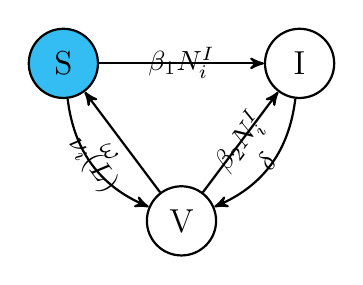
\begin{tikzpicture}[->, >=stealth', auto, thick, node distance=3cm]
                \tikzstyle{every state}=[fill=white,draw=black,thick,text=black,scale=1,font=\large]
    
                \node[state, fill=cyan!80!white] at (0, 0)  (S)  {S};
                \node[state] at (3, 0)  (I)  {I};
                \node[state] at (1.5, -2) (V)  {V};
        
                \path
                (S) edge[sloped] node[above, inner sep=0pt, yshift=-0.2cm]{$\beta_1 N^I_i$} (I)
        		(V) edge[sloped] node[above, inner sep=0pt, yshift=-0.3cm]{$\omega$} (S)
        		(S) edge[sloped, bend right=30] node[below, inner sep=0pt, yshift=0.2cm]{$\nu_i(L)$} (V)
                (I) edge[sloped, bend left=30] node[below, inner sep=0pt, yshift=0.2cm]{$\delta$} (V)
        		(V) edge[sloped] node[above, inner sep=0pt, yshift=-0.2cm]{$\beta_2 N^I_i$} (I);
            \end{tikzpicture}
        }
	
		\newcommand{\generateI}{%
		  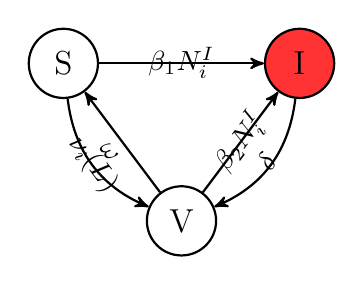
\begin{tikzpicture}[->, >=stealth', auto, thick, node distance=3cm]
				\tikzstyle{every state}=[fill=white,draw=black,thick,text=black,scale=1,font=\large]
				
				\node[state] at (0, 0)  (S)  {S};
				\node[state, fill=red!80!white] at (3, 0)  (I)  {I};
				\node[state] at (1.5, -2) (V)  {V};
				
				\path
                (S) edge[sloped] node[above, inner sep=0pt, yshift=-0.2cm]{$\beta_1 N^I_i$} (I)
        		(V) edge[sloped] node[above, inner sep=0pt, yshift=-0.3cm]{$\omega$} (S)
        		(S) edge[sloped, bend right=30] node[below, inner sep=0pt, yshift=0.2cm]{$\nu_i(L)$} (V)
                (I) edge[sloped, bend left=30] node[below, inner sep=0pt, yshift=0.2cm]{$\delta$} (V)
        		(V) edge[sloped] node[above, inner sep=0pt, yshift=-0.2cm]{$\beta_2 N^I_i$} (I);
		  \end{tikzpicture}
		}
	
		\newcommand{\generateV}{%
		  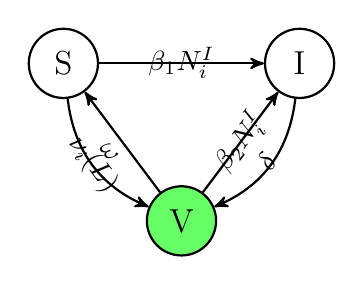
\begin{tikzpicture}[->, >=stealth', auto, thick, node distance=3cm]
				\tikzstyle{every state}=[fill=white,draw=black,thick,text=black,scale=1,font=\large]
				
				\node[state] at (0, 0)  (S)  {S};
				\node[state] at (3, 0)  (I)  {I};
				\node[state, fill=green!60!white] at (1.5, -2) (V)  {V};
				
				\path
                (S) edge[sloped] node[above, inner sep=0pt, yshift=-0.2cm]{$\beta_1 N^I_i$} (I)
        		(V) edge[sloped] node[above, inner sep=0pt, yshift=-0.3cm]{$\omega$} (S)
        		(S) edge[sloped, bend right=30] node[below, inner sep=0pt, yshift=0.2cm]{$\nu_i(L)$} (V)
                (I) edge[sloped, bend left=30] node[below, inner sep=0pt, yshift=0.2cm]{$\delta$} (V)
        		(V) edge[sloped] node[above, inner sep=0pt, yshift=-0.2cm]{$\beta_2 N^I_i$} (I);
		  \end{tikzpicture}
		}
	
		
		% Include the generated diagram code in the nodes
		\node[state] at (0, 0)  (n1)  {\resizebox{1cm}{!}{\generateS}};
		\node[state] at (3, 0)  (n2)  {\resizebox{1cm}{!}{\generateI}};
		\node[state] at (0, -2) (n3)  {\resizebox{1cm}{!}{\generateSS}};
		\node[state] at (3, -2) (n4)  {\resizebox{1cm}{!}{\generateV}};
		
		\path
		(n1) edge[sloped] node[above]{} (n2)
		(n1) edge[sloped] node[above]{} (n3)
		(n2) edge[sloped] node[above]{} (n3)
		(n2) edge[sloped] node[above]{} (n4);
	\end{tikzpicture}
\end{document}
